\subsection{Extreme dry heat: testing the efficiency ranking}
We test $T_a=T_r=40\,^{\circ}\mathrm C$ at RH 15\% and 20\%, retaining the device powers, delivery profiles, 5/8$\,^{\circ}\mathrm C$ outlet caps, and uniform occupancy. Figure~\ref{fig:extreme-heat} shows $\eta_A>\eta_B>\eta_C$ in both cases. At RH 15\%, the mean SET reductions are 1.43, 1.95, and 3.42$\,^{\circ}\mathrm C$, whereas the efficiencies are 68.43, 19.48, and 16.41 person$\cdot{}^{\circ}\mathrm C\cdot$h/kWh. C produces greater relief per passenger, but consumes ten times A's electricity. SET relief explains the service numerator; $\eta$ remains the comparison criterion.

The heat balance explains why dry-bulb cooling alone cannot establish the ranking. When air is warmer than the exposed skin or clothing surface, faster flow increases convective heat gain; it also promotes evaporative heat loss. SET combines these competing exchanges rather than imposing a temperature-triggered reversal of fan performance \cite{thermalcomfort}.

\begin{figure}[htbp]
\centering
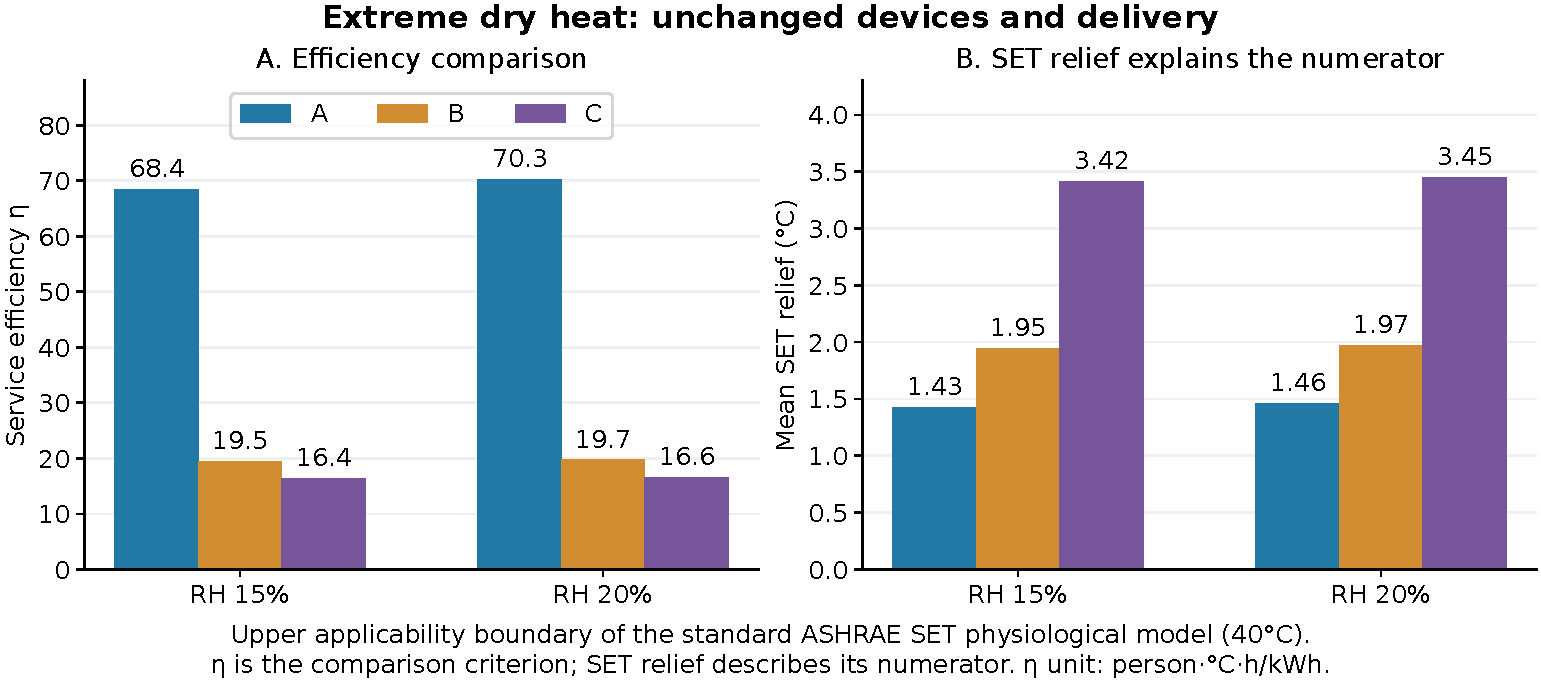
\includegraphics[width=0.85\textwidth]{figures/26_extreme_heat.pdf}
\caption{Extreme dry-heat boundary test with the original device powers and delivery profiles. The left panel compares cooling efficiency; the right panel explains its SET-relief numerator. Inputs follow Assumption A4.}
\label{fig:extreme-heat}
\end{figure}
